\begin{center}
 \textsf{Листок 3.}
\end{center}
\vspace{0.01cm}
\nopagebreak[2]
\task{
  Напряжённость однородного электрического поля равна $E$. Чему равен
  поток напряжённости электрического поля через квадрат со стороной
  $l$, плоскость которого расположена под углом $30^{o}$ к направлению
  поля? 
}
\task{
  Найдите отрицательные и положительные потоки однородного
  электрического поля напряжённости $E$ через замкнутую поверхность
  прямой трёхгранной призмы, высота которой $h$. Передняя грань
  призмы, ширина которой равна $h$, перпендикулярна $E$, нижняя грань
  параллельна $E$. 
}
\task{Используя теорему Гаусса, определите напряжённость
  электрического поля внутри и вне равномерно заряженной сферы, если
  полный заряд сферы $Q$; равномерно заряженной бесконечной нити, если
  заряд единицы длины равен $\rho$; вне и внутри равномерно заряженной
  бесконечной пластины толщиной $h$, если объёмная плотность заряда в
  пластине равна $\rho$.}
\task{
  Докажите теорему Ирншоу. 
}
\task{
  При пересечении двух шаров радиуса $R$, центры которых находятся на
  расстоянии $l$ друг от друга, образуются два <<полумесяца>>,
  равномерно заряженных разноимёнными электрическими
  зарядами. Объёмная плотность электрического заряда равна
  $\rho$. Докажите, что электрическое поле в области пересечения шаров
  однородно. Найдите его напряжённость. 
}

\taskpic{В равномерно заряженной бесконечной пластине вырезали
  сферическую полость так, как показано на рисунке. Толщина пластины
  $h$, объёмная плотность заряда $\rho$. Чему равна напряжённость
  электрического поля в точке $A$, в точке
  $B$?}{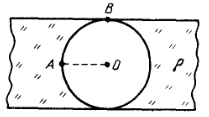
\includegraphics[width=4cm]{d10_3_1.png}}
\task{
  Две пересекающиеся под углом $\alpha$ бесконечные плоскости делят
  пространство на четыре области. Чему равна напряжённость
  электрического поля в этих областях, если поверхностная плотность
  заряда плоскостей $\pm \sigma$?
}